\documentclass[12pt]{article}
\usepackage[a4paper,margin=0.75in]{geometry}
\usepackage[utf8]{inputenc}
\usepackage[OT1]{fontenc}
\usepackage[table,usenames,dvipsnames]{xcolor}
\usepackage{array}
\usepackage{varwidth}
\usepackage{multirow,tabularx}
\usepackage{amsmath}
\usepackage{hyperref}
\usepackage{enumitem}
\usepackage{graphicx}
\usepackage{tcolorbox}
\renewcommand*\familydefault{\sfdefault}

\newtcolorbox{mybox}[3][]
{
  colframe = #2!25,
  colback  = #2!10,
  coltitle = #2!20!black,  
  title    = {#3},
  #1,
}

\hypersetup{
    colorlinks=true,
    linkcolor=blue,
    filecolor=magenta,      
    urlcolor=cyan,
    pdftitle={Overleaf Example},
    pdfpagemode=FullScreen,
}

\title{\textbf{COL774 Assignment 3}}
\author{Aniruddha Deb \\ \texttt{2020CS10869}}
\date{October 2022}

\begin{document}

\maketitle

\section{Decision Trees, Random Forests, Gradient Boosted Trees}

\subsection{Dataset 1}

\begin{enumerate}[label=(\alph*)]
    \item After removing the missing values, we obtain the following accuracies:
    \begin{enumerate}[label=(\roman*)]
        \item \textbf{Training set:} 92.53 \%
        \item \textbf{Validation set:} 76.03 \%
        \item \textbf{Test set:} 69.17 \%
    \end{enumerate}

    The decision tree we obtain is as follows (drawn upto a depth of 3):
    \begin{center}
        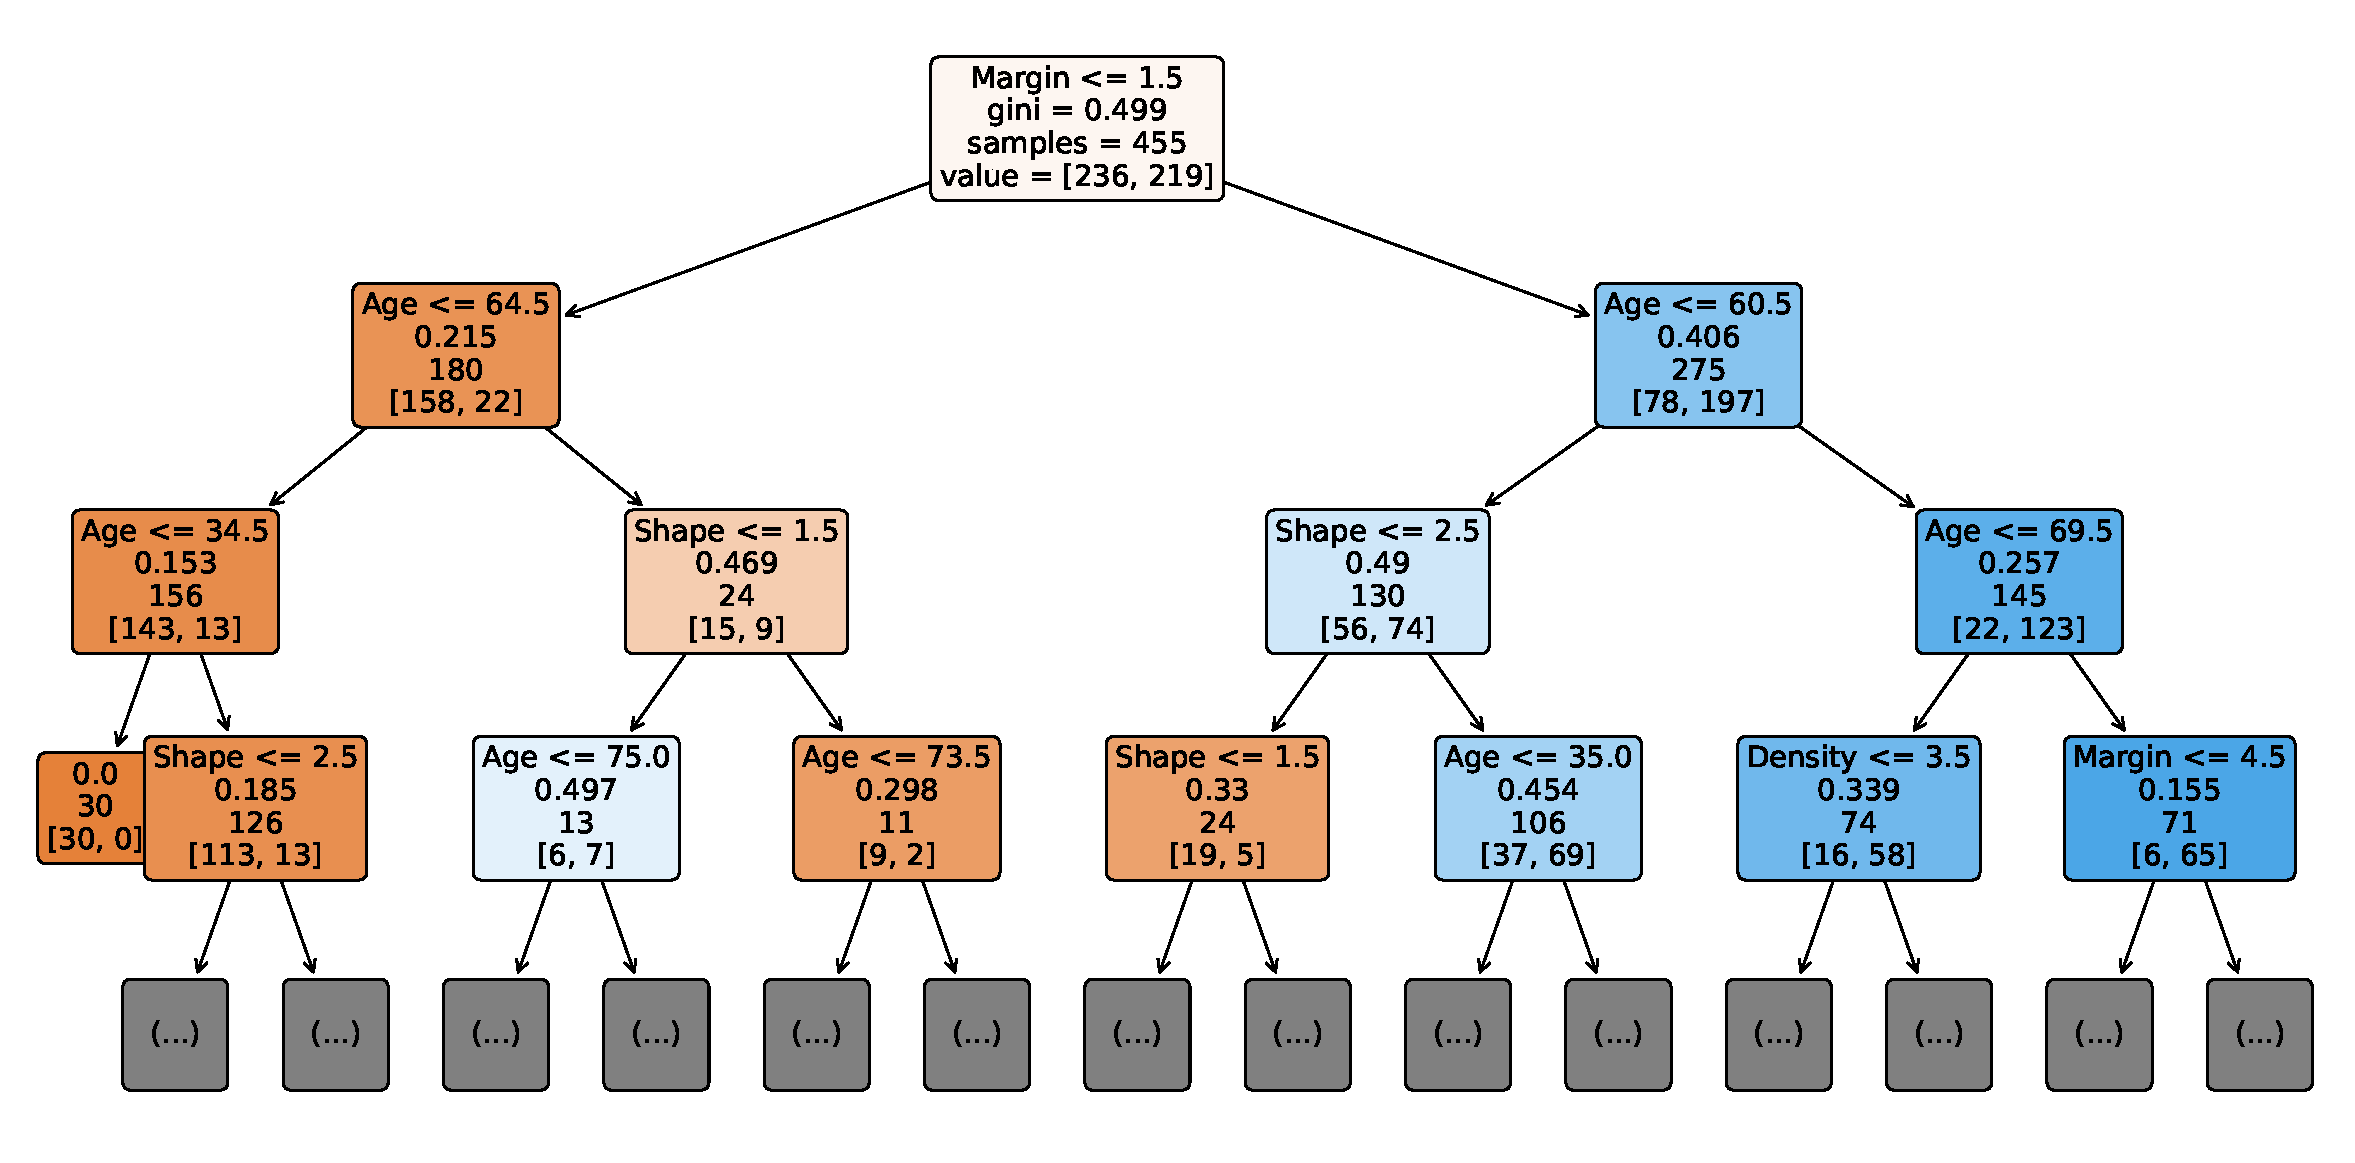
\includegraphics[width=0.94\textwidth]{../Q1/tree.pdf}
    \end{center}

    \item With GridSearchCV and the grid of parameters $\text{max\_depth}=\{4,6,8,10\}$, 
    $\text{min\_samples\_split}=\{2,3,4,5\}$ and $\text{min\_samples\_leaf}=\{1,2,3,4,5\}$,
    the best parameters (obtained via five-fold cross validation) are:
    \begin{enumerate}[label=(\roman*)]
        \item max\_depth = 4
        \item min\_samples\_leaf = 5
        \item min\_samples\_split = 2
    \end{enumerate}

    With them, we obtain the following accuracies:
    \begin{enumerate}[label=(\roman*)]
        \item \textbf{Training set:} 81.98 \%
        \item \textbf{Validation set:} 87.6 \%
        \item \textbf{Test set:} 75.1 \%
    \end{enumerate}

    The decision tree has a much shallower depth than the previous tree, and is
    also simpler

    \begin{center}
        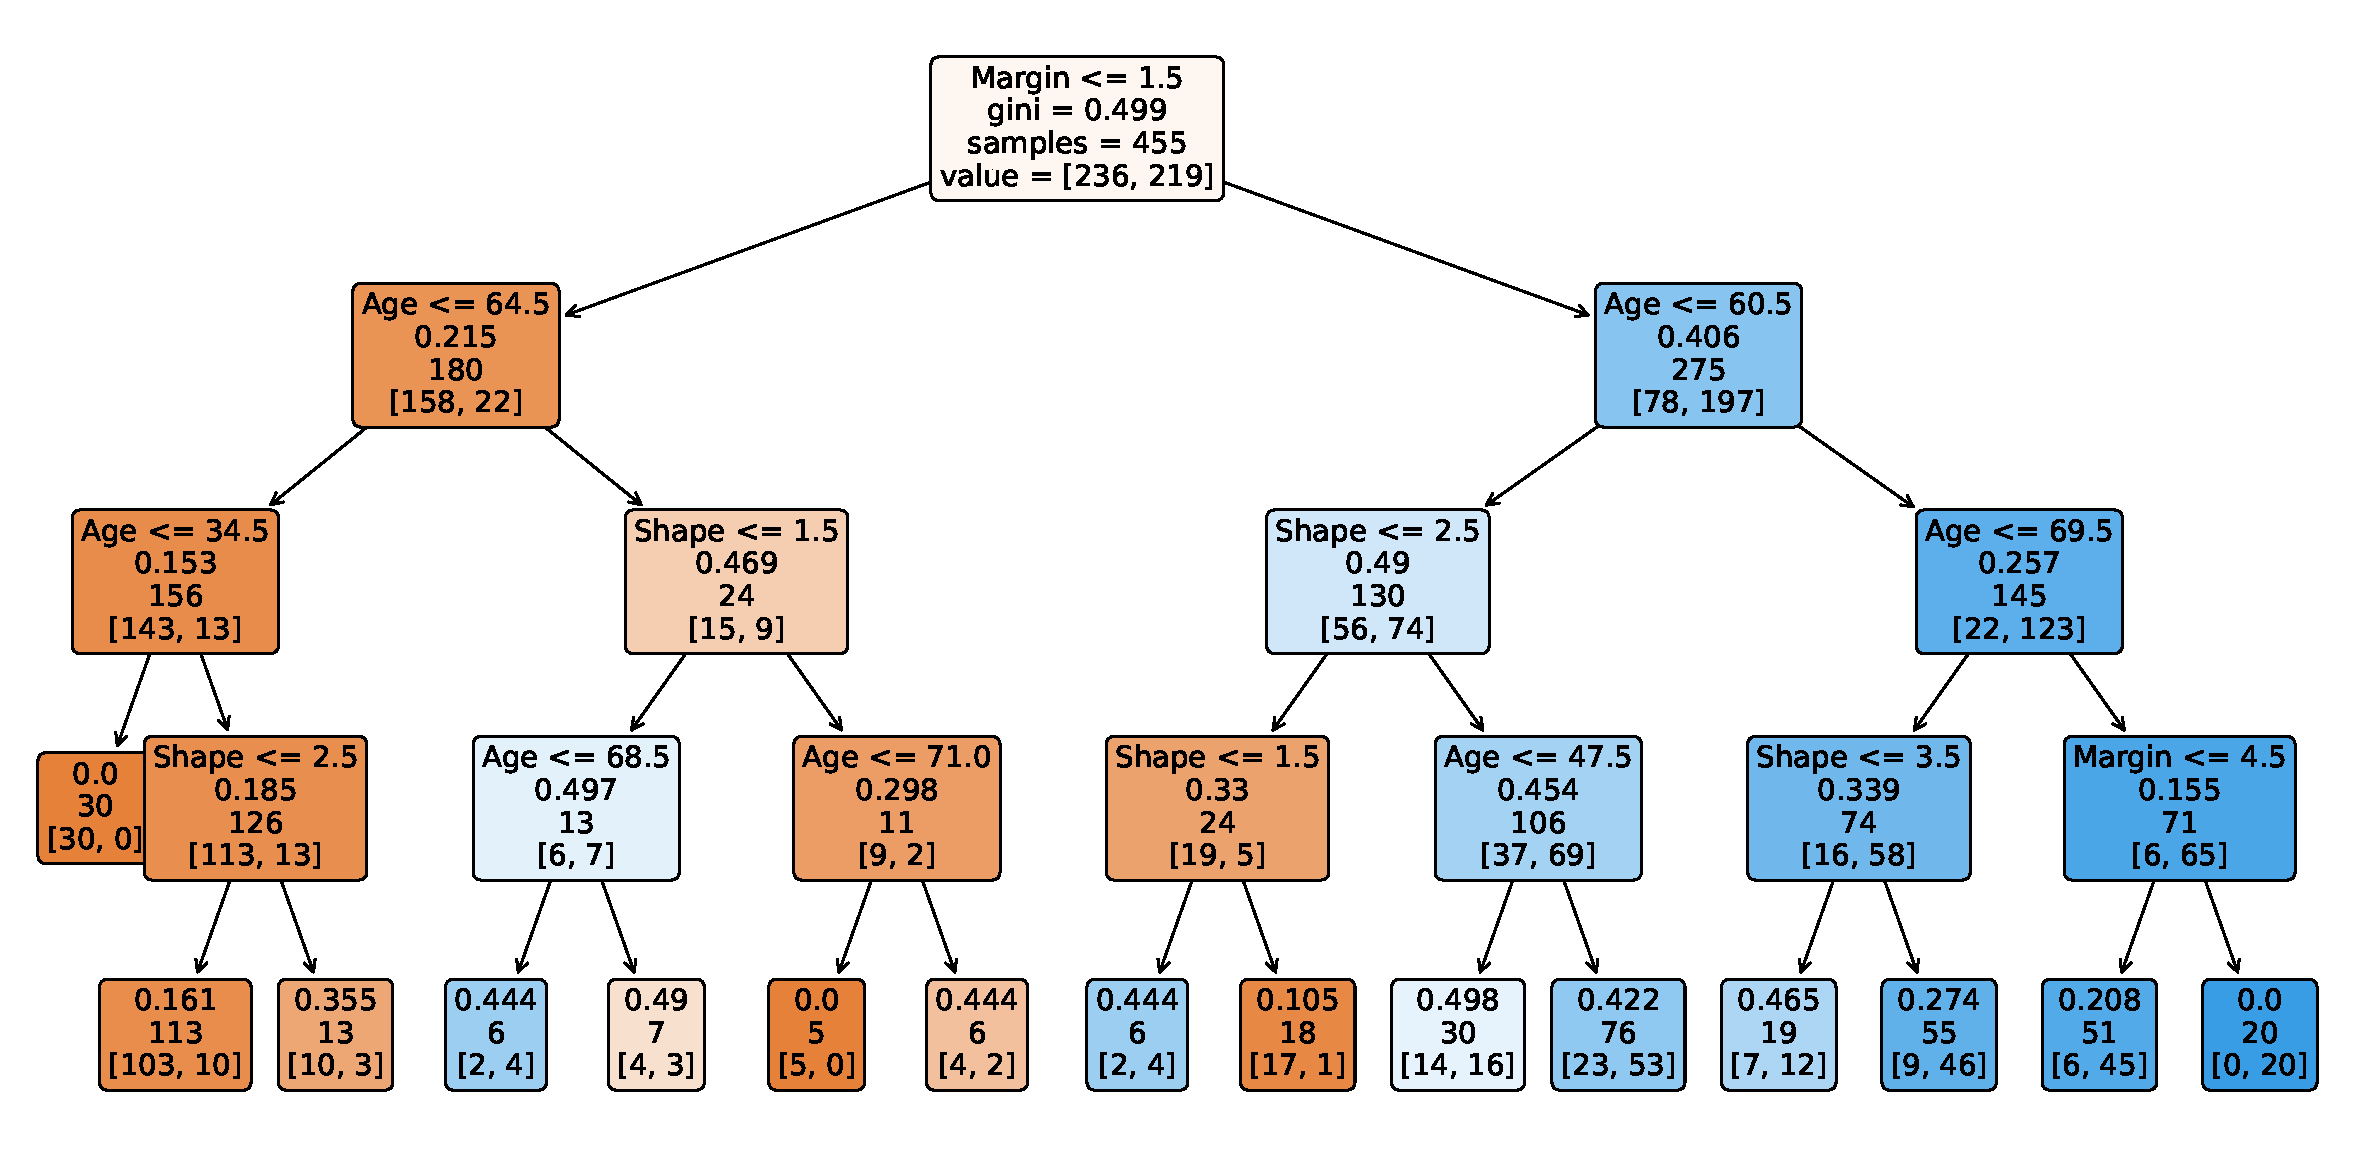
\includegraphics[width=0.94\textwidth]{../Q1/tree_optimal.pdf}
    \end{center}

    \item The total impurity vs the alphas is plotted below, along with the depth
        and the number of nodes v/s alpha

    \begin{center}
        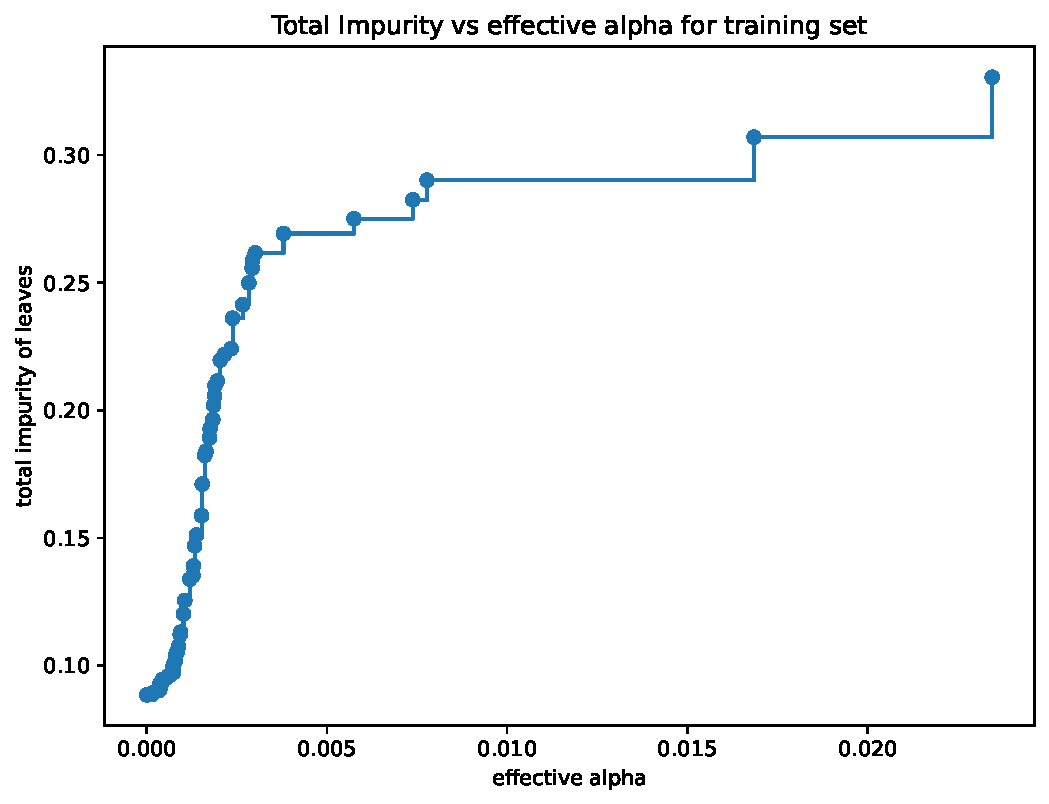
\includegraphics[width=0.45\textwidth]{../Q1/impurity_vs_alpha.pdf}
        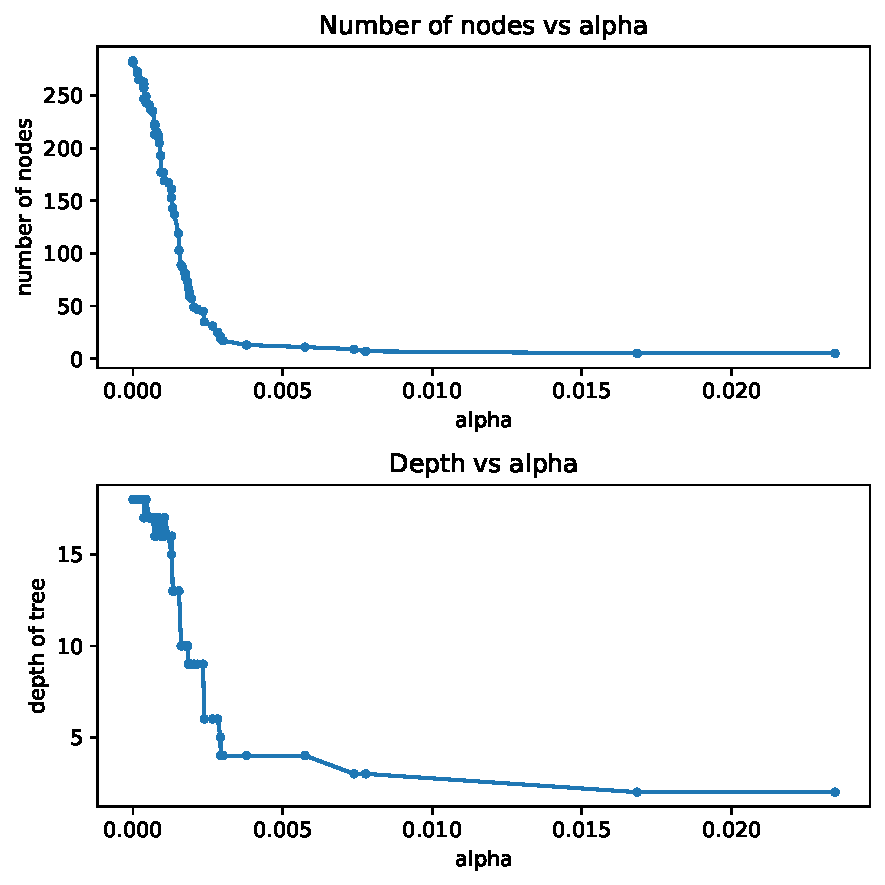
\includegraphics[width=0.45\textwidth]{../Q1/nodes_vs_alpha.pdf}
    \end{center}

    We see that the training accuracy is very high for low values of alpha, at 
    the expense of the validation and test accuracy i.e. the model overfits for 
    low values of alpha. The best trees are the ones with fewer nodes

    \begin{center}
        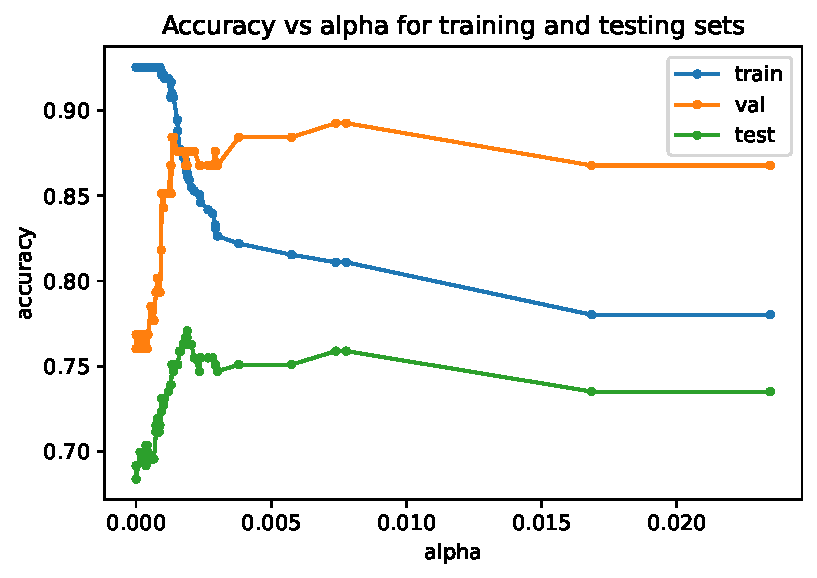
\includegraphics[width=0.6\textwidth]{../Q1/accuracy_vs_alpha.pdf}
    \end{center}

    The accuracies we obtain for the various datasets, using the best pruned tree
    are:
    \begin{enumerate}
        \item \textbf{Training set:} 81.1 \%
        \item \textbf{Validation set:} 89.26 \%
        \item \textbf{Test set:} 75.89 \%
    \end{enumerate}

    The best pruned tree, as discussed before, has only 9 nodes compared to the 
    trees we obtained in part (a) and part (b). 

    \begin{center}
        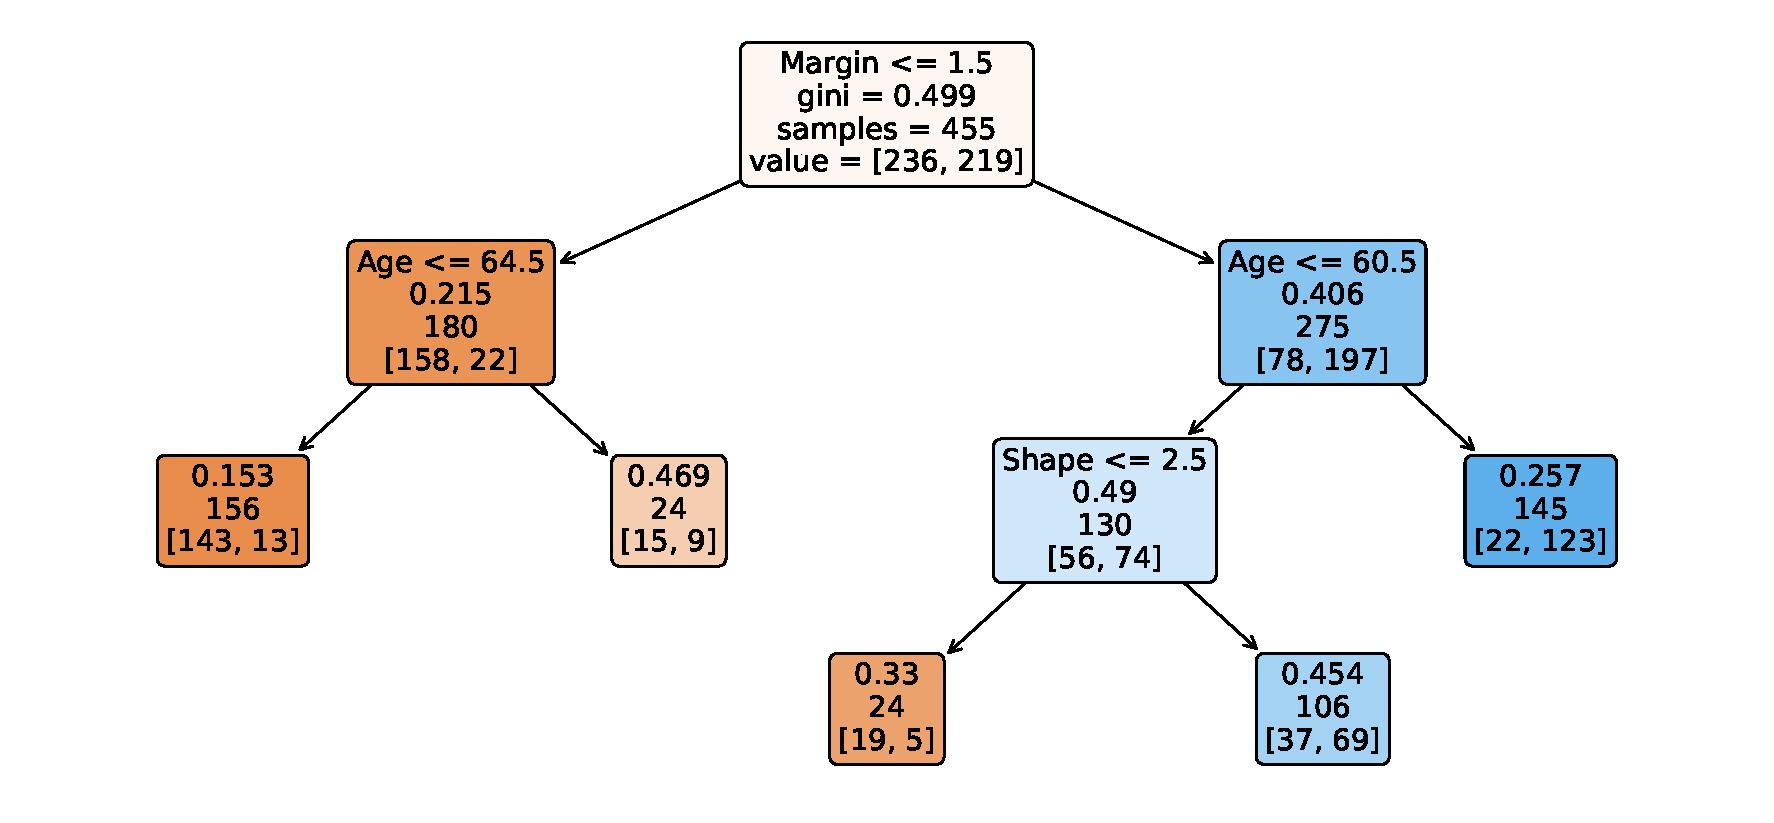
\includegraphics[width=0.94\textwidth]{../Q1/tree_best_pruned.pdf}
    \end{center}

    \item With GridSearchCV and the grid of parameters $\text{n\_estimators}=\{50, 100, 150, 200\}$, \\
    $\text{max\_features}=\{1,2,3,4\}$ and $\text{min\_samples\_split}=\{2,3,4,5\}$,
    the best parameters (obtained using out of bag score as the metric) are:
    \begin{enumerate}[label=(\roman*)]
        \item n\_estimators = 200
        \item min\_samples\_split = 5
        \item max\_features = 3
    \end{enumerate}

    With them, we obtain the following accuracies:
    \begin{enumerate}[label=(\roman*)]
        \item \textbf{Training set:} 90.11 \%
        \item \textbf{Out of Bag set:} 76.26 \%
        \item \textbf{Validation set:} 86.78 \%
        \item \textbf{Test set:} 76.68 \%
    \end{enumerate}

    \item The results are summarized in the following table:

    \begin{center}
    \begin{tabular}{l c c}
        Default decision tree: & Median & Mode \\
        \hline
        \hspace{3mm} Train & 91.81 \% & 90.69 \% \\
        \hspace{3mm} Validation & 74.07 \% & 75.56 \% \\
        \hspace{3mm} Test & 74.31 \% & 71.18 \% \\
             & & \\
        Grid Searched Decision tree: & Median & Mode \\
        \hline
        \hspace{3mm} max\_depth & 4 & 4 \\
        \hspace{3mm} min\_samples\_split \hspace{30mm} & 2 & 2 \\ % hack for some space
        \hspace{3mm} min\_samples\_leaf & 3 & 2 \\
        \hspace{3mm} Train & 81.56 \% & 81.38 \% \\
        \hspace{3mm} Validation & 87.41 \% & 86.67 \% \\
        \hspace{3mm} Test & 80.90 \% & 77.43 \% \\
            & & \\
        ccp\_alpha optimized Decision tree: & Median & Mode \\
        \hline
        \hspace{3mm} n\_nodes & 11 & 137 \\
        \hspace{3mm} ccp\_alpha & 0.0055 & 0.0012 \\
        \hspace{3mm} Train & 80.26 \% & 88.83 \% \\
        \hspace{3mm} Validation & 87.41 \% & 88.15 \% \\
        \hspace{3mm} Test & 79.17 \% & 76.04 \% \\
            & & \\
        Random Forest classifier: & Median & Mode \\
        \hline
        \hspace{3mm} n\_estimators & 200 & 100 \\
        \hspace{3mm} min\_samples\_split & 5 & 5 \\
        \hspace{3mm} max\_features & 3 & 2 \\
        \hspace{3mm} Train & 88.45 \% & 88.08 \% \\
        \hspace{3mm} Out of Bag & 75.23 \% & 73.37 \% \\
        \hspace{3mm} Validation & 83.70 \% & 83.70 \% \\
        \hspace{3mm} Test & 77.78 \% & 77.43 \% \\
    \end{tabular}
    \end{center}

    What do I see? Lot of gruntwork without any point % TODO give a good reason here
    
    \item After implementing an XGBoost classifier and searching for parameters
    using GridSearchCV in the given parameter space, we obtain the following 
    best parameters:
    \begin{enumerate}[label=(\roman*)]
        \item max\_depth = 10
        \item n\_estimators = 10
        \item subsample = 0.5
    \end{enumerate}

    With them, we obtain the following accuracies:
    \begin{enumerate}[label=(\roman*)]
        \item \textbf{Training set:} 83.61 \%
        \item \textbf{Validation set:} 84.44 \%
        \item \textbf{Test set:} 77.08 \%
    \end{enumerate}
\end{enumerate}

\subsection{Dataset 2}

\begin{enumerate}[label=(\alph*)]
    \item blah
\end{enumerate}
\end{document}
